\chapter{Design}
The system is designed to handle a substantial volume of data with varying attributes in both number and type. 
There are several anime and manga entries that contains missing or incomplete information, 
and the system must be able to handle this, avoiding meaningless memory occupation. To accommodate this, 
a Document Database was chosen for its flexibility and schema-less nature, ease of use, and high-performance 
capabilities. This choice enables the execution of complex queries, including advanced filtering across different attribute types.

\vspace{\baselineskip}

In addition, the implementation of social networking functionalities necessitated the use of a Graph Database. 
This allows for efficient traversal of relationships between entities and effectively manages connections between 
different entities such as users, anime, and manga.


\section{Document Database}

The decision to use a document database, specifically MongoDB,  was driven by its \textbf{flexibility} 
and \textbf{schema-less nature}, which allows for the storage of data with varying attributes in both number and type. 
This adaptability makes MongoDB ideal for handling diverse and dynamic data models.

\vspace{\baselineskip}

MongoDB also provides a \textbf{high-performance environment} for executing complex queries, 
reducing the need for joins and improving overall application performance by minimizing database 
access. This is particularly beneficial for applications like MangaVerse that require fast response 
times and can benefit from pre-computed relationships between entities. By storing embedded 
relationships directly within documents, MongoDB enables quicker data retrieval, enhancing user experience.

\vspace{\baselineskip}

To avoid normalized data, \textbf{data redundancy} is used to define relationships between entities.
Although this technique can lead to increased memory usage, it enables faster queries and fewer 
database accesses. For applications with high query complexity and rapidly growing data, 
such as MangaVerse, this is an optimal trade-off.

\vspace{\baselineskip}

To define \textbf{one-to-many relationships}, the documents linking pattern is used. 
In this pattern, one entity stores a list of the IDs of related entities, allowing for 
quick retrieval without multiple queries. This approach is used for retrieving reviews 
written by a user or reviews associated with a specific anime or manga. Additionally, document 
embedding is used for storing the latest reviews within the anime or manga documents, enabling 
fast access to this information when a user views the anime or manga page.

\vspace{\baselineskip}

The document database also includes other redundancies between collections and between the document
database and the graph database. For example, fields such as the number of likes for a manga or 
anime, the number of followers and followings for a user, and the average rating of media content
are stored redundantly. To maintain consistency without unnecessary database accesses, a flag 
called \textbf{'avg\_rating\_last\_update'} is used to indicate whether the average rating is 
up-to-date.

\vspace{\baselineskip}

MongoDB is also a \textbf{scalable database}, capable of handling large volumes of data and traffic. 
It supports distribution, providing \textbf{high availability}, \textbf{fault tolerance}, and \textbf{data integrity}. 
This means MongoDB can easily be scaled out to accommodate growth in both data and traffic, ensuring consistent 
performance and reliability as the application grows.


\vspace{\baselineskip}

\subsection*{Collections}
The database contains the following collections:
\begin{itemize}
    \item \textbf{Anime}: 
    This collection stores information about anime, including a list of review IDs and the most recent reviews as nested documents.
    
    \item \textbf{Manga}: 
    This collection stores information about manga, including a list of review IDs and the most recent reviews as nested documents.
    
    \item \textbf{Reviews}: 
    This collection stores user ratings and comments for media content. To enhance performance and reduce multiple queries, it 
    includes some user and media redundancies, especially for suggestions and analytics.
    
    \item \textbf{Users}: 
    This collection stores user data along with a list of review IDs.
\end{itemize}

\subsection*{Analytics and Suggestions}

The application performs various analytics on users, manga, and anime to provide the manager with valuable information 
regarding user distribution and the average rating of the application or media content. These analytics are grouped 
by different criteria such as genre, season, and year. Additionally, the application offers personalized 
media content suggestions to users.

\vspace{\baselineskip}

The following is a comprehensive list of all the queries that the application should be able to execute:

\vspace{\baselineskip}

\begin{itemize}
    \item \textbf{User Analytics}:
    \begin{itemize}
        \item Retrieve the distribution of users grouped by gender, joined\_on date, birthday, and country;
        \item Retrieve the average rating of the application grouped by gender, joined\_on date, birthday, and country;
    \end{itemize}
    
    \item \textbf{Media Content Analytics}:
    \begin{itemize}
        \item Retrieve the average rating of the media content grouped by various criteria (e.g., genre, type, demographics, author, etc.);
        \item Retrieve the average rating of a media content per month or year;
    \end{itemize}
    
    \item \textbf{Suggestions}:
    \begin{itemize} 
        \item Retrieve the top media content suggestions for a user based on the user's location or birthday.
    \end{itemize}
\end{itemize}
    
\subsection*{CRUD operations}
\begin{itemize}
  \item \textbf{CREATE}
  \begin{itemize}
      \item Create a user
      \item Create an anime
      \item Create a manga
      \item Create a review
  \end{itemize}

  \item \textbf{UPDATE}
  \begin{itemize}
      \item Update user's information
      \item Update media content details
      \item Update a review
  \end{itemize}

  \item \textbf{DELETE}
  \begin{itemize}
      \item Delete a user
      \item Delete a media content
      \item Delete a review by its ID
      \item Delete reviews of a user
      \item Delete reviews of a media content
      \item Delete reviews not related to any media content
      \item Delete a review not related to any user
  \end{itemize}

  \item \textbf{READ}
  \begin{itemize}
      \item Read a user by the ID
      \item Read the first N users by username
      \item Read a media content by its ID
      \item Read a page of media contents by filters
      \item Read reviews of a specified user
      \item Read reviews of a specified media content
  \end{itemize}
\end{itemize}

\subsection*{JSON document example}
Anime:
\begin{lstlisting}[language=json]
{
  _id: {
    $oid: "65789bb52f5d29465d0abcfc"
  },
  title: "\"Aesop\" no Ohanashi yori: Ushi to Kaeru, Yokubatta Inu",
  type: "MOVIE",
  "episodes": 1,
  status: "FINISHED",
  picture: "https://cdn.myanimelist.net/images/anime/3/65151.jpg",
  tags: [
    "family friendly",
    "fantasy",
    "frogs",
    "kids"
  ],
  synopsis: "Based on Aesop's Fables.",
  latest_reviews: [
    {
      id: {
        $oid: "657ed1b40481d3954cf8d69c"
      },
      comment: "Struggles to maintain interest; fails to captivate.",
      date: {
        $date: "2022-04-11T22:00:00.000Z"
      },
      user: {
        id: {
          $oid: "6577877ce683762347607f42"
        },
        username: "dreadstuff",
        picture: "https://imgbox.com/7MaTkBQR"
      }
    },
    {
      id: {
        $oid: "657ebc340481d3954cf842e5"
      },
      comment: "Wouldn't recommend to even the most forgiving viewers.",
      date: {
        $date: "2021-03-19T23:00:00.000Z"
      },
      user: {
        id: {
          $oid: "6577877ce683762347606bc6"
        },
        username: "Yoma_Yuki",
        picture: "https://imgbox.com/7MaTkBQR"
      }
    }
  ],
  anime_season: {
    season: "WINTER",
    year: 1970
  },
  average_rating: 4.5,
  avg_rating_last_update: true,
  review_ids: [
    "66695c50222b3184dbb7d990",
    "66695c50222b3184dbb7d991",
    "66695c50222b3184dbb7d992"
  ],
  likes: 7
}\end{lstlisting}

Manga:
\begin{lstlisting}[language=json]
{
  _id: {
    $oid: "657ac61cb34f5514b91eabc1"
  },
  title: "H20",
  type: "MANHWA",
  status: "FINISHED",
  volumes: 7,
  chapters: 43,
  genres: [
    "Romance",
    "Slice of Life"
  ],
  demographics: [
    "SHOUJO"
  ],
  authors: [
    {
      id: 4354,
      role: "Story & Art",
      name: "Sook Ji Hwang"
    }
  ],
  serializations: "Wink",
  synopsis: "Menga is simply known as the vice rep and is bullied. Hanako has moved to Korea but was robbed the first day and has nothing. Na Hong Soo is known as a troublemaker and is in constant trouble. And Eechan is the student body president, very popular and known as Bacchus. It seems they have nothing in common but this will change soon. \n\n(Source: mangaupdates.com)",
  title_english: "H20",
  picture: "https://cdn.myanimelist.net/images/manga/1/1053l.jpg",
  average_rating: 3.67,
  latest_reviews: [
    {
      id: {
        $oid: "66682d94bebc20d9557bba39"
      },
      comment: "Beautiful artwork and engaging characters.",
      date: {
        $date: "2024-06-17T21:33:37.000Z"
      },
      rating: 7,
      user: {
        id: {
          $oid: "6577877be68376234760635b"
        },
        username: "Sanji-kun",
        picture: "images/account-icon.png"
      }
    },
    {
      id: {
        $oid: "66682d94bebc20d9557bba35"
      },
      comment: "An average manga with a few standout moments.",
      date: {
        $date: "2024-02-10T20:53:52.000Z"
      },
      rating: 7,
      user: {
        id: {
          $oid: "6577877ce6837623476065f0"
        },
        username: "MangoSlushie",
        picture: "https://thypix.com/wp-content/uploads/2021/10/manga-profile-picture-92.jpg"
      }
    }
  ],
  start_date: null,
  end_date: null,
  avg_rating_last_update: true,
  review_ids: [
    "66682d94bebc20d9557bba35",
    "66682d94bebc20d9557bba36",
    "66682d94bebc20d9557bba3b"
  ]
}\end{lstlisting}


Reviews:
\begin{lstlisting}[language=json]
{
  _id: {
    $oid: "66682a4fbebc20d9557b7542"
  },
  user: {
    id: {
      $oid: "6577877ce683762347607b2f"
    },
    username: "dagdffsfgf",
    location: "Singapore",
    birthday: {
      $date: "1991-02-12T00:00:00.000Z"
    }
  },
  manga: {
    id: {
      $oid: "657ac61bb34f5514b91ea22a"
    },
    title: "Kaguya-sama wa Kokurasetai: Tensai-tachi no Renai Zunousen"
  },
  rating: 9,
  comment: "Rich in emotion and excitement.",
  date: {
    $date: "2022-07-18T07:18:21.000Z"
  }
}\end{lstlisting}

Users:
\begin{lstlisting}[language=json]
{
  _id: {
    $oid: "6577877be683762347605859"
  },
  email: "xdavis@example.com",
  password: "290cb38a679d5eb68d11b9ea1e21f48234eba6de19f95612dbcb70ce0c7e4e78",
  description: "Liberating the mind from stress with the power of anime zen.",
  picture: "https://thypix.com/wp-content/uploads/2021/10/manga-profile-picture-44.jpg",
  username: "Xinil",
  gender: "Male",
  birthday: {
    $date: "1985-03-04T00:00:00.000Z"
  },
  location: "South Africa",
  joined_on: {
    $date: "2016-11-30T00:00:00.000Z"
  },
  app_rating: 1,
  followed: 40,
  followers: 29,
  review_ids: [
    "66682a5cbebc20d9557b76b5",
    "66682b31bebc20d9557b8886",
    "66682e66bebc20d9557bcb29",
    "66683301bebc20d9557bf017"
  ]
}\end{lstlisting}

\subsection*{Redundancy}

In a document database, data redundancy can be leveraged to enhance application performance and reduce the
number of database accesses. However, the application must manage the consistency between the original data
and their redundant copies. This consistency maintenance can impact performance and availability. Therefore,
optimal strategies are necessary to ensure data consistency while preserving application performance and availability.

\vspace{\baselineskip}

The following redundancies are implemented in the database:

\vspace{\baselineskip}

\begin{itemize}
    \item \textbf{Latest Reviews}: \\
    In the anime and manga collections, a field contains the latest 5 reviews for that specific media content. This approach ensures fast retrieval.

    \vspace{\baselineskip}

    \item \textbf{Average Rating}: \\
    In the anime and manga collections, a field contains the average rating of the media content. This field is updated every time a new review is written.

    \vspace{\baselineskip}

    \item \textbf{Number of Likes}: \\
    In the anime and manga collections, a field contains the number of likes. This field is updated every time a new like relationship is created or deleted.

    \vspace{\baselineskip}

    \item \textbf{Followers and Followings}: \\
    In the user collection, fields contain the number of followers and followings. These fields are updated every time a new follow relationship is created or deleted.

    \vspace{\baselineskip}

    \item \textbf{User Field in Reviews}: \\
    In the reviews collection, a field contains user data, such as id, username, picture, location, and birthday. This data is used for suggestion purposes.

    \vspace{\baselineskip}

    \item \textbf{Media Content Field in Reviews}: \\
    In the reviews collection, a field contains information about the anime or manga the review pertains to, including the media content id and title.

    \vspace{\baselineskip}

    \item \textbf{Review Ids}: \\
    A list of review ids is stored in the anime, manga, and user collections. This list is used to quickly retrieve the reviews of media content and users.
\end{itemize}

\newpage

\section{Graph Database}

The inclusion of social networking functionalities, such as user interactions, likes, and follows, necessitated the 
integration of a graph database to efficiently manage relationships between entities. A graph database operates on 
the concepts of nodes and relationships, which are ideal for this purpose. Unlike traditional databases that rely on 
join tables—often resulting in higher memory usage and slower execution times due to multiple database accesses—a graph 
database optimizes traversal for relationships. This makes it particularly well-suited for managing complex connections 
between users, anime, and manga, ensuring faster and more efficient data retrieval and manipulation.

\vspace{\baselineskip}

Additionally, graph databases provide enhanced flexibility and scalability, allowing for easier implementation of 
new features and relationships as the application grows. They support advanced queries that can traverse multiple 
relationships in a single operation, offering a significant performance boost for social networking applications 
where interconnected data is prevalent.

\begin{figure}[htbp]\label{fig:GraphDB}
  \centering
  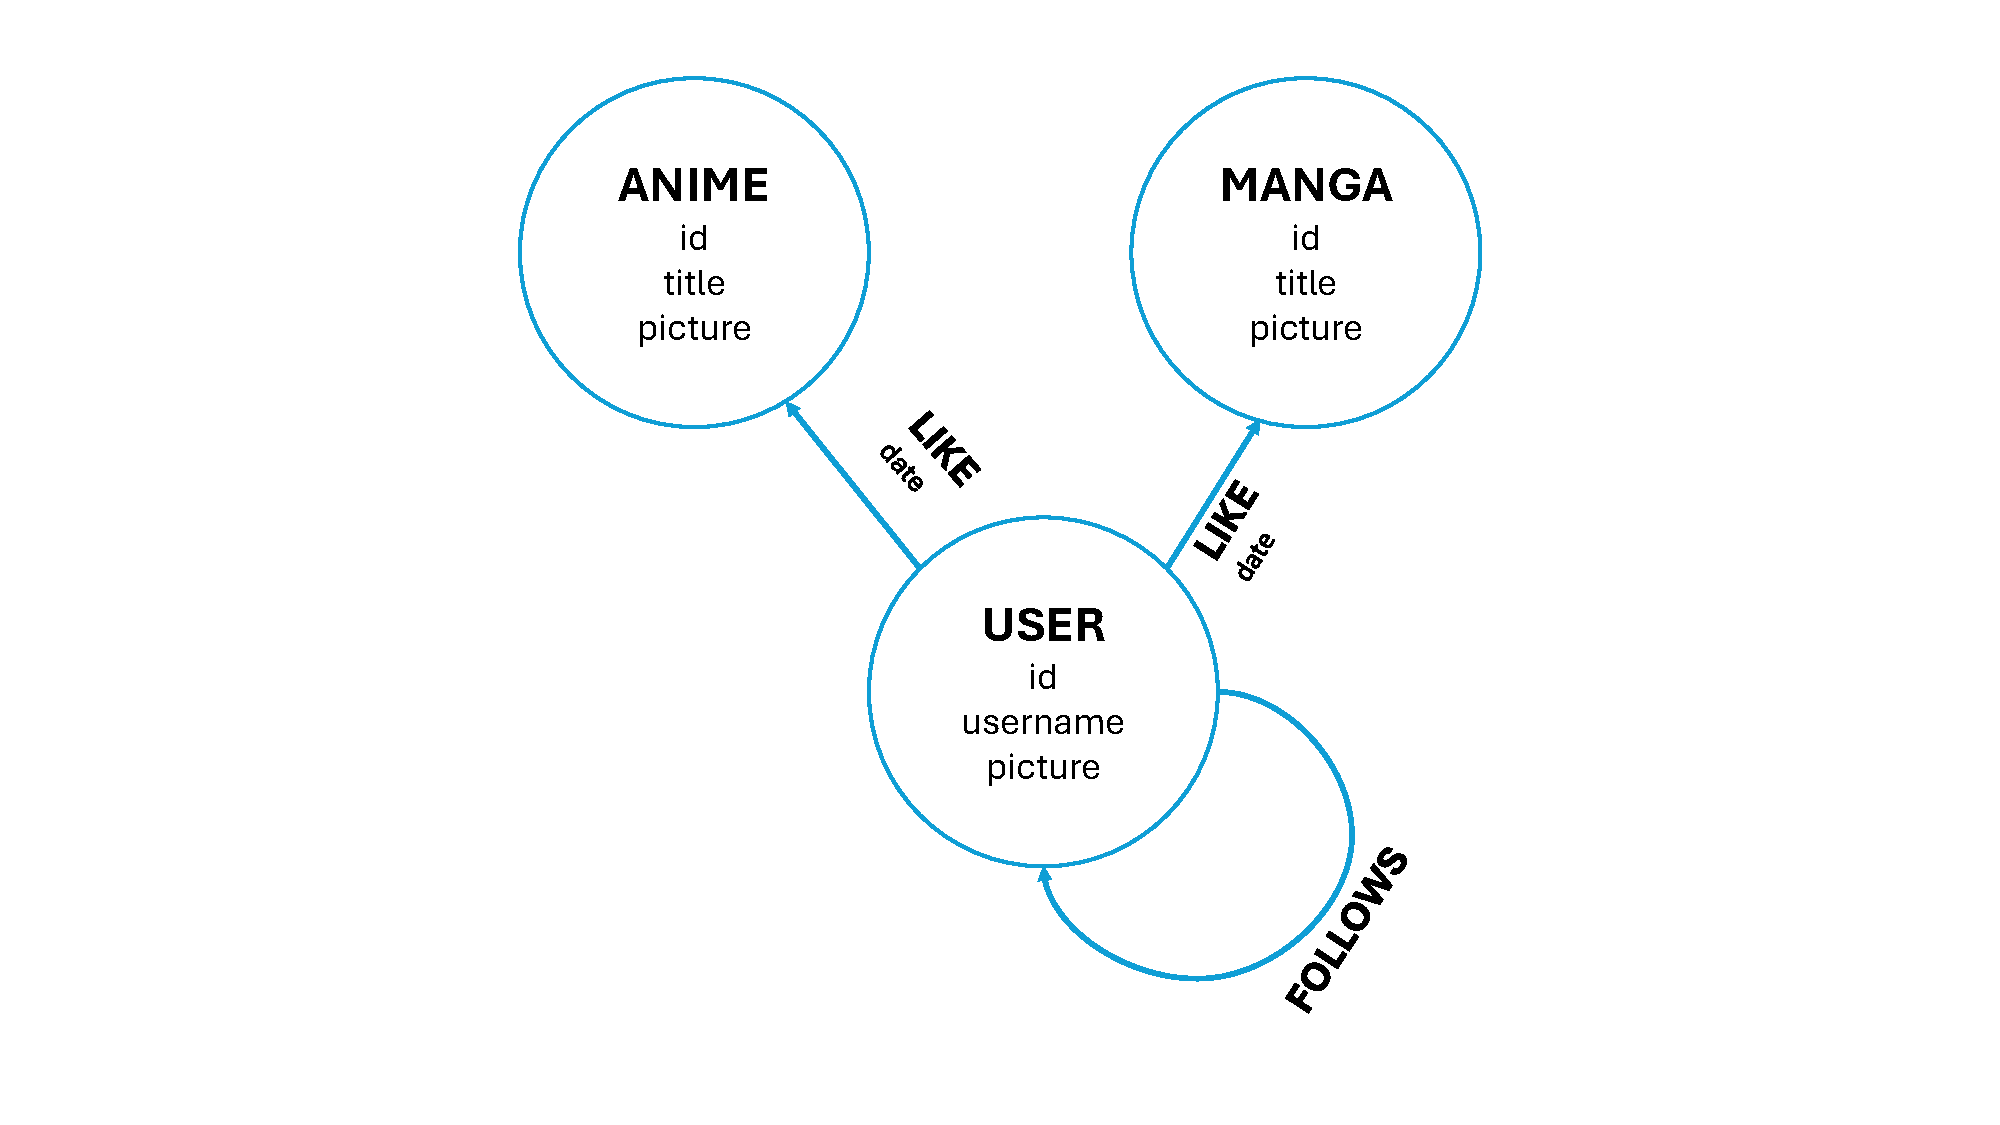
\includegraphics[width=0.9\textwidth]{Media/graph.pdf}
\end{figure}

\newpage

\subsection*{Nodes}

The database will have the following nodes:
\begin{itemize}
    \item User: This node will store information about users, such as id, usernames, and picture.
    \item Anime: This node will store information about anime, such as id, titles and picture.
    \item Manga: This node will store information about manga, such as id, titles and picture.
\end{itemize}

\subsection*{Relationships}

The database will have the following relationships:
\begin{itemize}
    \item LIKE\@: This relationship will connect users to anime and manga nodes. It will store the date when the user liked the media content.
    \item FOLLOW\@: This relationship will connect users to other users. 
\end{itemize}

\subsection*{CRUD operations}
\begin{itemize}
  \item \textbf{CREATE}
  \begin{itemize}
      \item Create a user node
      \item Create an anime node
      \item Create a manga node
      \item Create a LIKE edge between a user and an anime or manga
      \item Create a FOLLOW edge between two users
  \end{itemize}

  \item{UPDATE}
  \begin{itemize}
      \item Update user's picture and/or username
      \item Update media content picture and/or title
  \end{itemize}

  \item{DELETE}
  \begin{itemize}
      \item Delete a user node and all edge connected to it
      \item Delete a media content node and all edge connected to it
      \item Delete a LIKE edge between a user and an anime or manga
      \item Delete a FOLLOW edge between two users
  \end{itemize}

  \item{READ}
  \begin{itemize}
    \item Read the numer of FOLLOW edges outcoming from a user
    \item Read the number of FOLLOW edges incoming to a user
    \item Read the number of LIKE edges incoming to an anime or manga
    \item Read the list of followers of a user
    \item Read the list of followings of a user
  \end{itemize}
\end{itemize}

\section{Availability and Partition Tolerance (AP)}

MangaVerse, as a social network, adopts the AP configuration of the CAP theorem, emphasizing Availability
and Partition Tolerance. This ensures users can reliably access the application, interact with others,
and engage with media content, even though data consistency may vary (Eventual Consistency).
This approach enhances user experience by prioritizing uninterrupted service over strict data consistency.

\section{Replicas}

For MangaVerse, three MongoDB replicas were deployed to ensure high availability, partition tolerance,
and rapid response times. This configuration allows the system to remain accessible and responsive even
during network partitions or node failures. However, managing data consistency across multiple replicas
requires careful handling to achieve eventual consistency without compromising availability.

\section{Sharding}

Even though sharding is not currently implemented in MangaVerse, it's crucial to consider its implications.
Sharding is a method used to distribute data across multiple machines, essential for managing data growth.
As datasets expand, a single machine may become inadequate for storing and managing data with acceptable
read and write speeds. Document databases like MongoDB support sharding, which facilitates horizontal scaling.

\vspace{\baselineskip}

Choosing the right shard key for each collection is critical for effective sharding in MongoDB\@.
The shard key determines how data is distributed across shards. Factors such as the types of queries performed,
document relationships, and document structure must be carefully evaluated when selecting a shard key to ensure
optimal performance and scalability.

\vspace{\baselineskip}

In its current implementation, MangaVerse does not support sharding. A potential approach could involve sharding
anime and manga data by unique identifiers like id or title, and reviews by media content id or title to keep
related data together on the same shard. However, this strategy may lead to performance challenges. Queries
involving reviews related to a specific user or media content suggestions based on user location and birthday
could require accessing multiple shards, potentially reducing application performance. Similarly, analytical
tasks like computing average ratings across anime and manga collections would necessitate querying all shards,
which can be inefficient.